% move all configuration stuff into includes file so we can focus on the content
\documentclass[aspectratio=169,hyperref={pdfpagelabels=false,colorlinks=true,linkcolor=white,urlcolor=lightblue},xcolor={table},t]{beamer}

%%%%%%%%%%%%%%%%%%%%%%%%%%%%%%%%%%%%%%%%%%%%%%%%%%%%%%%%%%%%%%%%%%%%%%%%%%%%%%%%%%
%%%%%%%%%%%%%%%%%%%%%%%%%%%%%%%%%%%%%%%%%%%%%%%%%%%%%%%%%%%%%%%%%%%%%%%%%%%%%%%%%%
% packages
\usepackage{pict2e}
\usepackage{epic}
\usepackage{amsmath,amsfonts,amssymb}
\usepackage{units}
\usepackage{fancybox}
\usepackage[absolute,overlay]{textpos} 
%\usepackage[table]{xcolor}
\usepackage{animate}
\usepackage{gensymb}
%\usepackage{graphicx}
%\usepackage{longtable}
\usepackage{multirow}
\usepackage{silence}
\usepackage{tikz}
\usepackage[backend=bibtex,style=ieee]{biblatex}
\AtEveryCitekey{\iffootnote{\tiny}{}}
\addbibresource{include/references}



% fontsize
\let\Tiny=\tiny

%%%%%%%%%%%%%%%%%%%%%%%%%%%%%%%%%%%%%%%%%%%%%%%%%%%%%%%%%%%%%%%%%%%%%%%%%%%%%%%%%%
%%%%%%%%%%%%%%%%%%%%%%%%%%%%%%%%%%%%%%%%%%%%%%%%%%%%%%%%%%%%%%%%%%%%%%%%%%%%%%%%%%
% warnings
\pdfsuppresswarningpagegroup=1
\WarningFilter{biblatex}{Patching footnotes failed}
\WarningFilter{latexfont}{Font shape}
\WarningFilter{latexfont}{Some font shapes}
\WarningFilter{gensymb}{Not defining}


%%%%%%%%%%%%%%%%%%%%%%%%%%%%%%%%%%%%%%%%%%%%%%%%%%%%%%%%%%%%%%%%%%%%%%%%%%%%%%%%%%
%%%%%%%%%%%%%%%%%%%%%%%%%%%%%%%%%%%%%%%%%%%%%%%%%%%%%%%%%%%%%%%%%%%%%%%%%%%%%%%%%%
% theme & layout
\usetheme{Frankfurt}
\useinnertheme{rectangles}


%%%%%%%%%%%%%%%%%%%%%%%%%%%%%%%%%%%%%%%%%%%%%%%%%%%%%%%%%%%%%%%%%%%%%%%%%%%%%%%%%%
\setbeamertemplate{frametitle}[default][colsep=-4bp,rounded=false,shadow=false]
\setbeamertemplate{frametitle}
{%
    \nointerlineskip%
    %\vskip-0.5ex
    \begin{beamercolorbox}[wd=\paperwidth,ht=3.5ex,dp=0.6ex]{frametitle}
        \hspace*{1.3ex}\insertframetitle%
        
        \hspace*{1.3ex}\small\insertframesubtitle%
    \end{beamercolorbox}%
    \begin{textblock*}{100mm}(13.75cm,1cm)
        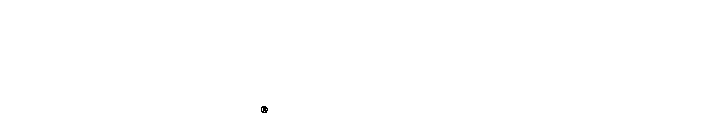
\includegraphics[height=.4cm,keepaspectratio]{graph/Logo_GTCMT_white}
    \end{textblock*}
}


%%%%%%%%%%%%%%%%%%%%%%%%%%%%%%%%%%%%%%%%%%%%%%%%%%%%%%%%%%%%%%%%%%%%%%%%%%%%%%%%%%
\setbeamertemplate{title page}[default][colsep=-4bp,rounded=false,shadow=false]
\setbeamertemplate{title page}
{
    \begin{textblock*}{100mm}(15cm,.51cm)
            \href{https://github.com/alexanderlerch/ACA-Slides/blob/2nd_edition/\jobname.pdf}{\includegraphics[height=.5cm,keepaspectratio]{graph/Logo_github}}\hspace*{2ex}
    \end{textblock*}
    \begin{textblock*}{100mm}(15cm,1.3cm)
            \href{\IEEELink}{
\includegraphics[height=.5cm,keepaspectratio]{graph/icon/book}}\hspace*{2ex}
    \end{textblock*}
    \vskip-10ex
    \begin{beamercolorbox}[wd=\paperwidth,ht=.7\paperheight,dp=0.6ex]{frametitle} %35ex
        %\begin{flushright}
            %\href{http://www.gtcmt.gatech.edu}{
\includegraphics[height=.8cm,keepaspectratio]{graph/Logo_GTCMT_black}}\hspace*{2ex}
        %\end{flushright}
        
        \hspace*{1.8ex}\LARGE\inserttitle%
        
        \vspace*{.5ex}
        
        \hspace*{1.3ex}\small\insertsubtitle%
        
        \vspace*{.5ex}
    \end{beamercolorbox}%
    \nointerlineskip%
    \begin{beamercolorbox}[wd=\paperwidth,ht=.4\paperheight,dp=0.6ex]{page number in head/foot}
        %\vspace*{-.5ex}
        \hspace*{1.7ex}\small\insertauthor%
        
        %\hspace*{1.7ex}\small }%
        
        \vspace*{12ex}
        \vfill
        \begin{flushright}
            \href{http://www.gtcmt.gatech.edu}{
\includegraphics[height=.5cm,keepaspectratio]{graph/Logo_GTCMT_black}}\hspace*{2ex}
        \end{flushright}
    \end{beamercolorbox}%
}


%%%%%%%%%%%%%%%%%%%%%%%%%%%%%%%%%%%%%%%%%%%%%%%%%%%%%%%%%%%%%%%%%%%%%%%%%%%%%%%%%%
%\makeatother
\setbeamertemplate{footline}
{
  \leavevmode%
  \hbox{%
  \begin{beamercolorbox}[wd=.5\paperwidth,ht=2.25ex,dp=1ex,left,leftskip=1ex]{page number in head/foot}%
    \insertsubtitle
  \end{beamercolorbox}%
  \begin{beamercolorbox}[wd=.5\paperwidth,ht=2.25ex,dp=1ex,right,rightskip=1ex]{page number in head/foot}%
    \hfill
    \insertframenumber{} / \inserttotalframenumber
  \end{beamercolorbox}}%
  \vskip0pt%
}
%\makeatletter


%%%%%%%%%%%%%%%%%%%%%%%%%%%%%%%%%%%%%%%%%%%%%%%%%%%%%%%%%%%%%%%%%%%%%%%%%%%%%%%%%%
\beamertemplatenavigationsymbolsempty
\setbeamertemplate{navigation symbols}{}
\setbeamertemplate{blocks}[default]%[rounded=false,shadow=false]
\setbeamertemplate{itemize item}[square]
\setbeamertemplate{itemize subitem}[circle]
\setbeamertemplate{itemize subsubitem}[triangle]
\setbeamertemplate{enumerate item}[square]
\setbeamertemplate{enumerate subitem}[circle]
\setbeamertemplate{enumerate subsubitem}[circle]


%%%%%%%%%%%%%%%%%%%%%%%%%%%%%%%%%%%%%%%%%%%%%%%%%%%%%%%%%%%%%%%%%%%%%%%%%%%%%%%%%%
% colors
\setbeamercolor{structure}{fg=darkgray}
\setbeamercovered{transparent} %invisible
\setbeamercolor{bibliography entry author}{fg=black}
\setbeamercolor*{bibliography entry title}{fg=black}
\setbeamercolor*{bibliography entry note}{fg=black}
\setbeamercolor{frametitle}{fg=black}
\setbeamercolor{title}{fg=white}
\setbeamercolor{subtitle}{fg=white}
\setbeamercolor{frametitle}{fg=white}
\setbeamercolor{framesubtitle}{fg=white}
\setbeamercolor{mini frame}{fg=white, bg=black}
\setbeamercolor{section in head/foot}{fg=white, bg=darkgray}
\setbeamercolor{page number in head/foot}{fg=black, bg=lightblue}
\setbeamercolor{item projected}{fg=white, bg=black}

%---------------------------------------------------------------------------------
%%%%%%%%%%%%%%%%%%%%%%%%%%%%%%%%%%%%%%%%%%%%%%%%%%%%%%%%%%%%%%%%%%%%%%%%%%%%%%%%%%
%%%%%%%%%%%%%%%%%%%%%%%%%%%%%%%%%%%%%%%%%%%%%%%%%%%%%%%%%%%%%%%%%%%%%%%%%%%%%%%%%%
% title information
\title[]{Introduction to \textbf{Audio Content Analysis}}   
\author[alexander lerch]{alexander lerch} 
%\institute{~}
%\date[Alexander Lerch]{}
%\titlegraphic{\vspace{-16mm}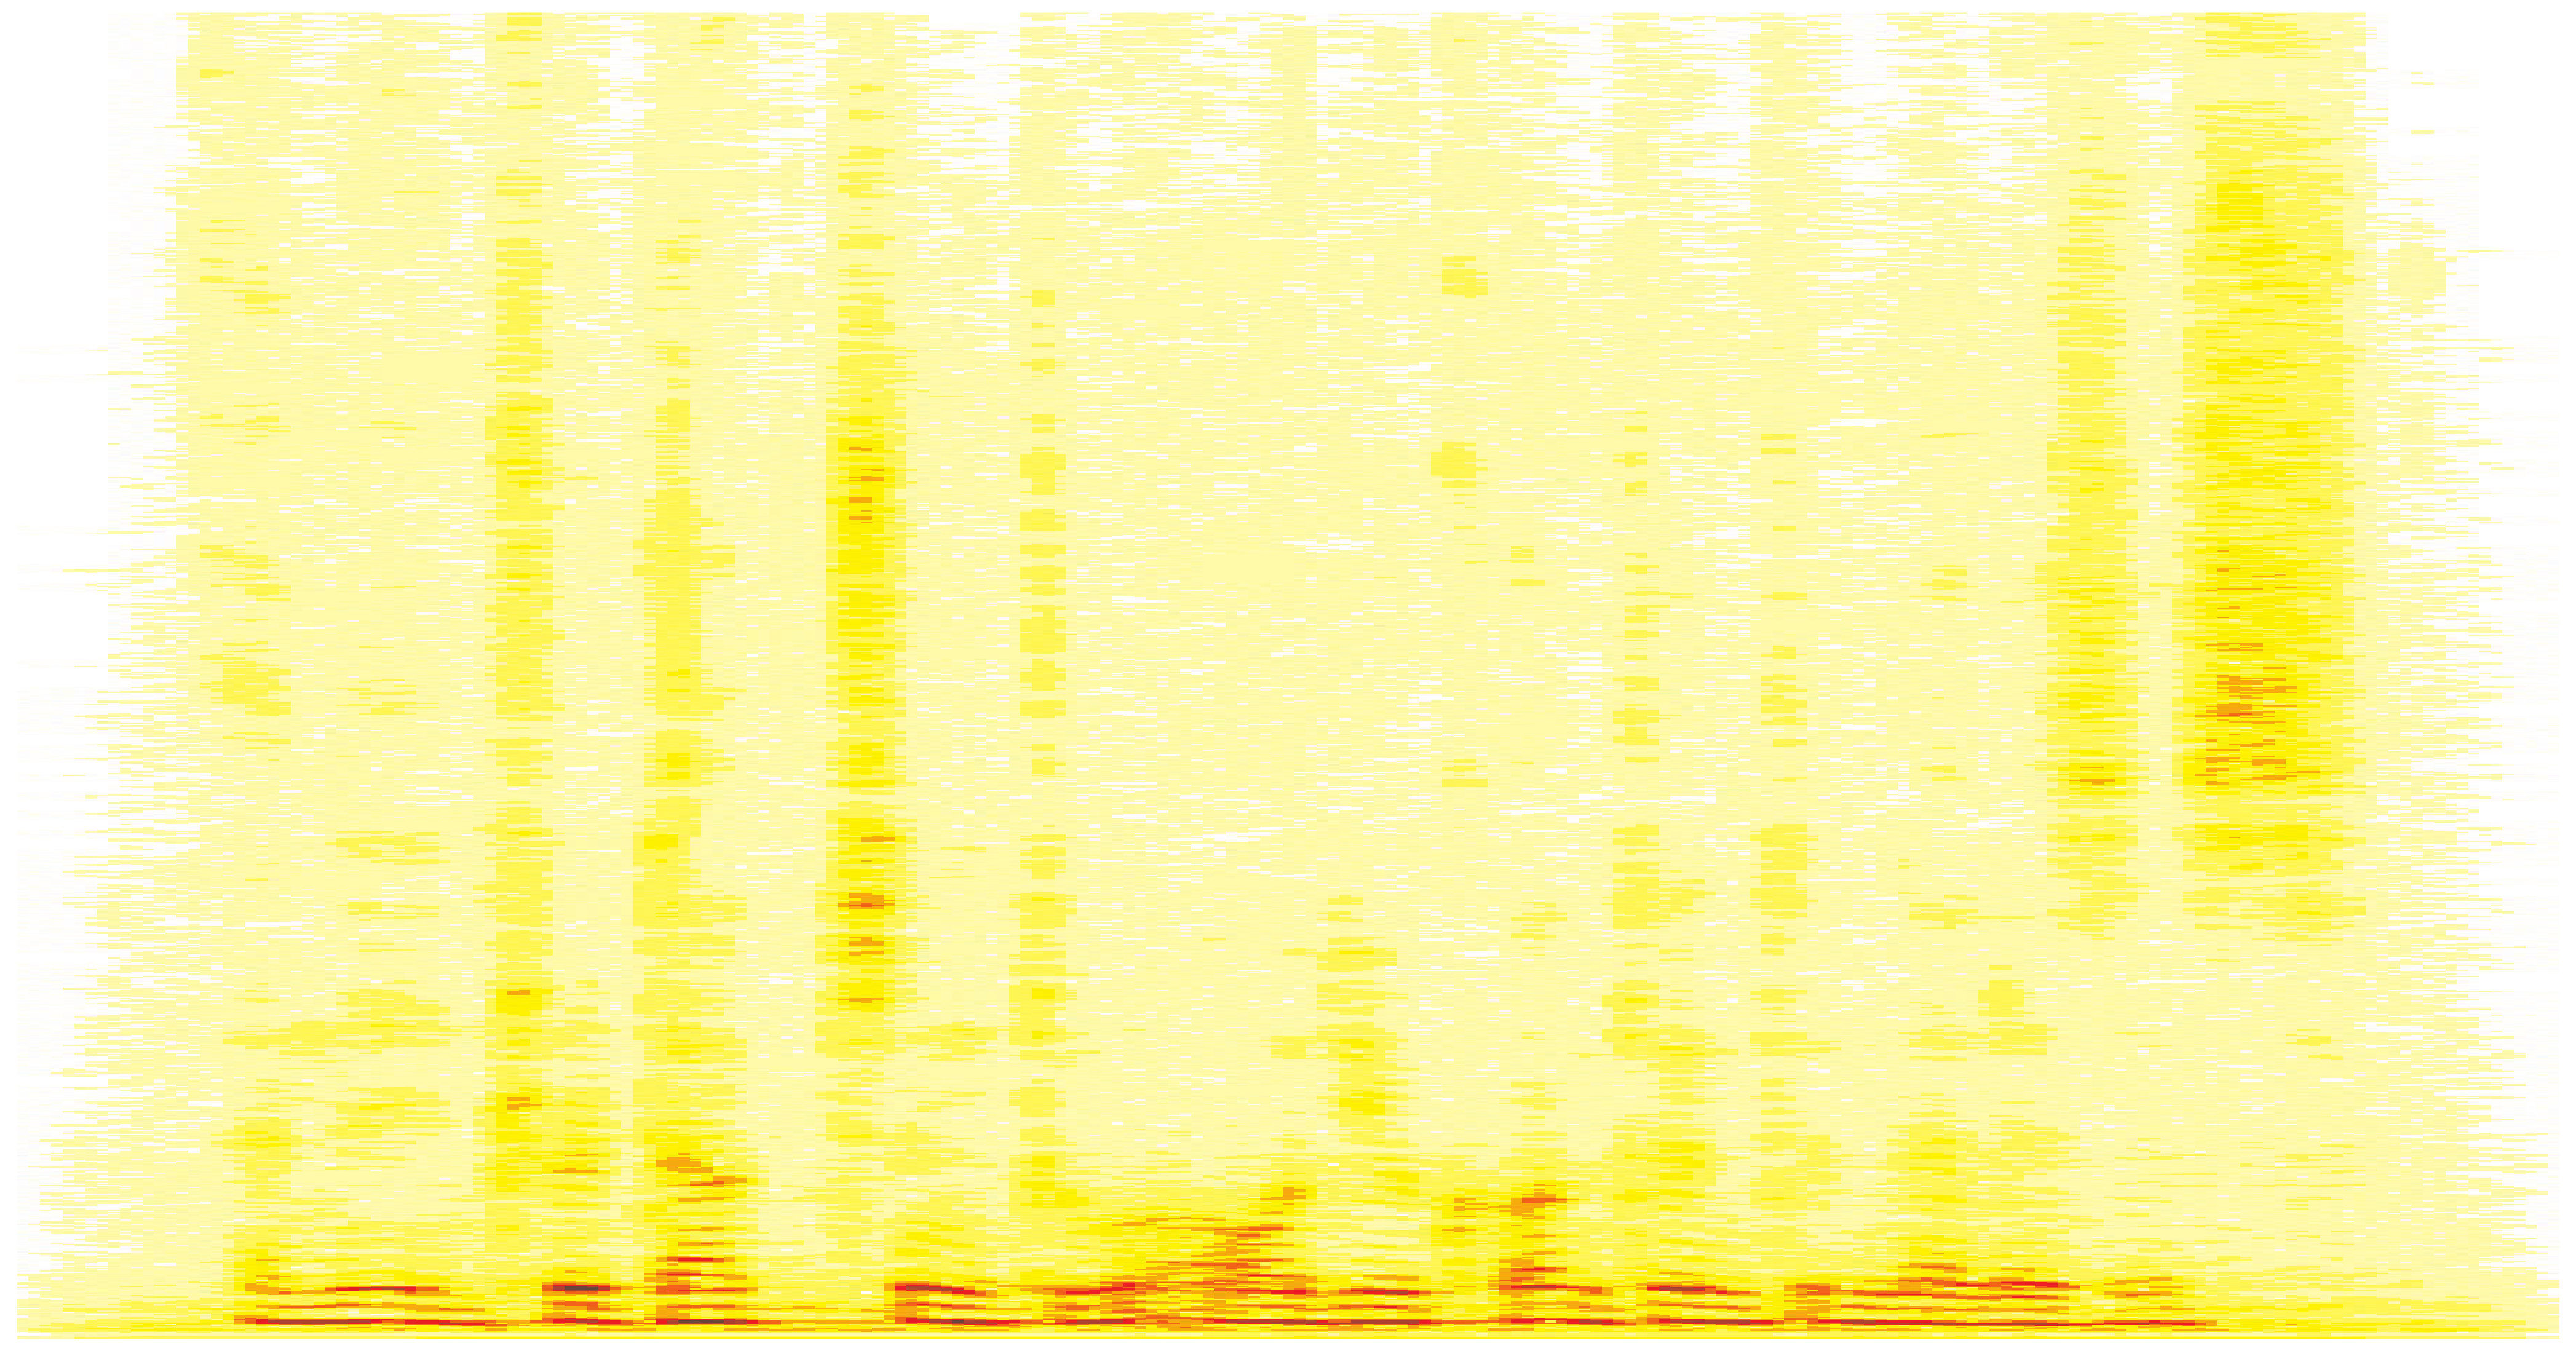
\includegraphics[width=\textwidth,height=3cm]{title}}

%%%%%%%%%%%%%%%%%%%%%%%%%%%%%%%%%%%%%%%%%%%%%%%%%%%%%%%%%%%%%%%%%%%%%%%%%%%%%%%%%%
%%%%%%%%%%%%%%%%%%%%%%%%%%%%%%%%%%%%%%%%%%%%%%%%%%%%%%%%%%%%%%%%%%%%%%%%%%%%%%%%%%
% colors
\definecolor{gtgold}{HTML}{96caff} %0e7eed {rgb}{0.88,0.66,1,0.06} [234, 170, 0]/256
\definecolor{darkgray}{rgb}{.1, .1, .25}
\definecolor{lightblue}{HTML}{0e7eed}
\definecolor{highlight}{rgb}{0, 0, 1} %_less!40

%%%%%%%%%%%%%%%%%%%%%%%%%%%%%%%%%%%%%%%%%%%%%%%%%%%%%%%%%%%%%%%%%%%%%%%%%%%%%%%%%%
%%%%%%%%%%%%%%%%%%%%%%%%%%%%%%%%%%%%%%%%%%%%%%%%%%%%%%%%%%%%%%%%%%%%%%%%%%%%%%%%%%
% relative paths
\graphicspath{{../ACA-Plots/graph/}}


%%%%%%%%%%%%%%%%%%%%%%%%%%%%%%%%%%%%%%%%%%%%%%%%%%%%%%%%%%%%%%%%%%%%%%%%%%%%%%%%%%
%%%%%%%%%%%%%%%%%%%%%%%%%%%%%%%%%%%%%%%%%%%%%%%%%%%%%%%%%%%%%%%%%%%%%%%%%%%%%%%%%%
% units
\setlength{\unitlength}{1mm}

%%%%%%%%%%%%%%%%%%%%%%%%%%%%%%%%%%%%%%%%%%%%%%%%%%%%%%%%%%%%%%%%%%%%%%%%%%%%%%%%%%
%%%%%%%%%%%%%%%%%%%%%%%%%%%%%%%%%%%%%%%%%%%%%%%%%%%%%%%%%%%%%%%%%%%%%%%%%%%%%%%%%%
% math
\DeclareMathOperator*{\argmax}{argmax}
\DeclareMathOperator*{\argmin}{argmin}
\DeclareMathOperator*{\atan}{atan}
\DeclareMathOperator*{\arcsinh}{arcsinh}
\DeclareMathOperator*{\sign}{sign}
\DeclareMathOperator*{\tcdf}{tcdf}
\DeclareMathOperator*{\si}{sinc}
\DeclareMathOperator*{\princarg}{princarg}
\DeclareMathOperator*{\arccosh}{arccosh}
\DeclareMathOperator*{\hwr}{HWR}
\DeclareMathOperator*{\flip}{flip}
\DeclareMathOperator*{\sinc}{sinc}
\DeclareMathOperator*{\floor}{floor}
\newcommand{\e}{{e}}
\newcommand{\jom}{\mathrm{j}\omega}
\newcommand{\jOm}{\mathrm{j}\Omega}
\newcommand   {\mat}[1]    		{\boldsymbol{\uppercase{#1}}}		%bold
\renewcommand {\vec}[1]    		{\boldsymbol{\lowercase{#1}}}		%bold

%%%%%%%%%%%%%%%%%%%%%%%%%%%%%%%%%%%%%%%%%%%%%%%%%%%%%%%%%%%%%%%%%%%%%%%%%%%%%%%%%%
%%%%%%%%%%%%%%%%%%%%%%%%%%%%%%%%%%%%%%%%%%%%%%%%%%%%%%%%%%%%%%%%%%%%%%%%%%%%%%%%%%
% media9
\newcommand{\includeaudio}[1]{
\href{run:audio/#1.mp3}{
\includegraphics[width=5mm, height=5mm]{graph/SpeakerIcon}}}

\newcommand{\includeanimation}[4]{{\begin{center}
                        \animategraphics[autoplay,loop,scale=.7]{#4}{animation/#1-}{#2}{#3}        
                        \end{center}
                        \addreference{matlab source: \href{https://github.com/alexanderlerch/ACA-Plots/blob/master/matlab/animate#1.m}{matlab/animate#1.m}}}
                        \inserticon{video}}
                        
%%%%%%%%%%%%%%%%%%%%%%%%%%%%%%%%%%%%%%%%%%%%%%%%%%%%%%%%%%%%%%%%%%%%%%%%%%%%%%%%%%
%%%%%%%%%%%%%%%%%%%%%%%%%%%%%%%%%%%%%%%%%%%%%%%%%%%%%%%%%%%%%%%%%%%%%%%%%%%%%%%%%%
% other commands
\newcommand{\question}[1]{%\vspace{-4mm}
                          \setbeamercovered{invisible}
                          \begin{columns}[T]
                            \column{.9\textwidth}
                                \textbf{#1}
                            \column{.1\textwidth}
                                \vspace{-8mm}
                                \begin{flushright}
                                     
\includegraphics[width=.9\columnwidth]{graph/question_mark}
                                \end{flushright}
                                \vspace{6mm}
                          \end{columns}\pause\vspace{-12mm}}

\newcommand{\toremember}[1]{
                        \inserticon{lightbulb}
                        }

\newcommand{\matlabexercise}[1]{%\vspace{-4mm}
                          \setbeamercovered{invisible}
                          \begin{columns}[T]
                            \column{.8\textwidth}
                                \textbf{matlab exercise}: #1
                            \column{.2\textwidth}
                                \begin{flushright}
                                     
\includegraphics[scale=.5]{graph/logo_matlab}
                                \end{flushright}
                                %\vspace{6mm}
                          \end{columns}}

\newcommand{\addreference}[1]{  
                  
                    \begin{textblock*}{\baselineskip }(.98\paperwidth,.5\textheight) %(1.15\textwidth,.4\textheight)
                         \begin{minipage}[b][.5\paperheight][b]{1cm}%
                            \vfill%
                             \rotatebox{90}{\tiny {#1}}
                        \end{minipage}
                   \end{textblock*}
                    }
                    
\newcommand{\figwithmatlab}[1]{
                    \begin{figure}
                        \centering
                        \includegraphics[scale=.7]{#1}
                        %\label{fig:#1}
                    \end{figure}
                    
                    \addreference{matlab source: \href{https://github.com/alexanderlerch/ACA-Plots/blob/main/matlab/plot#1.m}{plot#1.m}}}
\newcommand{\figwithref}[2]{
                    \begin{figure}
                        \centering
                        \includegraphics[scale=.7]{#1}
                        \label{fig:#1}
                    \end{figure}
                    
                    \addreference{#2}}  
                                    
\newcommand{\inserticon}[1]{
                    \begin{textblock*}{100mm}(14.5cm,7.5cm)
                        \includegraphics[height=.8cm,keepaspectratio]{graph/#1}
                    \end{textblock*}}            

%%%%%%%%%%%%%%%%%%%%%%%%%%%%%%%%%%%%%%%%%%%%%%%%%%%%%%%%%%%%%%%%%%%%%%%%%%%%%%%%%%
%%%%%%%%%%%%%%%%%%%%%%%%%%%%%%%%%%%%%%%%%%%%%%%%%%%%%%%%%%%%%%%%%%%%%%%%%%%%%%%%%%
% counters
\newcounter{i}
\newcounter{j}
\newcounter{iXOffset}
\newcounter{iYOffset}
\newcounter{iXBlockSize}
\newcounter{iYBlockSize}
\newcounter{iYBlockSizeDiv2}
\newcounter{iXBlockSizeDiv2}
\newcounter{iDistance}

\newcommand{\IEEELink}{https://ieeexplore.ieee.org/servlet/opac?bknumber=9965970}




\subtitle{module 9.5: tempo detection}

%%%%%%%%%%%%%%%%%%%%%%%%%%%%%%%%%%%%%%%%%%%%%%%%%%%%%%%%%%%%%%%%%%%%%%%%%%%%
\begin{document}
    % generate title page
	{
\setbeamertemplate{headline}{} 
\setbeamertemplate{footline}{} 
\begin{frame}
    \titlepage
    %\vspace{-5mm}
\end{frame}
}
\addtocounter{framenumber}{-1}


    \section[overview]{lecture overview}
        \begin{frame}{introduction}{overview}
            \begin{block}{corresponding textbook section}
                    %\href{http://ieeexplore.ieee.org/xpl/articleDetails.jsp?arnumber=6331123}{Chapter 6~---~Temporal Analysis}: pp.~146--148
                    section~9.5
            \end{block}

            \begin{itemize}
                \item   \textbf{lecture content}
                    \begin{itemize}
                        \item   introduction to tempo detection and beat tracking
                        \item   overview over basic approaches
                        \item    typical challenges
                    \end{itemize}
                \bigskip
                \item<2->   \textbf{learning objectives}
                    \begin{itemize}
                        \item   discuss advantages and disadvantages for different approaches to tempo detection and beat tracking
                        \item   summarize the typical challenges of beat tracking systems
                    \end{itemize}
            \end{itemize}
            \inserticon{directions}
        \end{frame}

    \section[intro]{introduction}
        \begin{frame}{tempo detection \& beat tracking}{problem statement}
            \begin{itemize}
                \item   \textbf{tempo detection}
                    \begin{itemize}
                        \item   detect speed of regular pulse (foot-tapping rate)
                    \end{itemize}
                \bigskip
                \item   \textbf{beat tracking}
                    \begin{itemize}
                        \item   detect the time instances the tempo pulses occur (beat phase)
                    \end{itemize}
            \end{itemize}
        \end{frame}
        
        \begin{frame}{tempo detection \& beat tracking}{introduction}
            \vspace{-3mm}
            \begin{columns}
            \column{.4\linewidth}
            \begin{itemize}
                \item \textbf{objectives}
                    \begin{enumerate}
                        \item	find the tempo from the novelty function/onsets
                        \item	find the beat locations
                    \end{enumerate}
                \bigskip
                \item \textbf{systematic problems}:
                    \begin{enumerate}
                        \item	distinguish \textit{hierarchical levels}
                            \begin{itemize}
                                \item	meter
                                \item	beat
                                \item	subbeat/tatum
                            \end{itemize}
                        \item<1->	detect \textit{beats without onsets}
                        \item<1->	recognize \textit{onsets without beats}
                    \end{enumerate}
            \end{itemize}
            \column{.6\linewidth}
                \figwithmatlab{BeatGrid}
            \end{columns}
        \end{frame}
        
        \begin{frame}{tempo detection \& beat tracking}{typical beat tracking system}
        \begin{figure}
        \scalebox{.75}{
			\centering
			\begin{footnotesize}
	\begin{picture}(100,70)
		\setcounter{iXBlockSize}{32}
		\setcounter{iYBlockSize}{16}
		\setcounter{iYBlockSizeDiv2}{8}
		\setcounter{iXBlockSizeDiv2}{16}
		\setcounter{iDistance}{8}

        % left branch top to bottom
		\setcounter{iYOffset}{48}
		\setcounter{iXOffset}{0}
		\addtocounter{iXOffset}{7}
		\addtocounter{iYOffset}{2}
		\put(\value{iXOffset}, \value{iYOffset})
			{\text{{\shortstack[c]{Audio/Midi\\ Signal}}}}
		\addtocounter{iXOffset}{-7}
		\addtocounter{iYOffset}{-2}
		
		\addtocounter{iXOffset}{\value{iXBlockSizeDiv2}}
        \put(\value{iXOffset}, \value{iYOffset})
			{\vector(0,-1){\value{iDistance}}}
		\addtocounter{iXOffset}{-\value{iXBlockSizeDiv2}}

		\addtocounter{iYOffset}{-\value{iDistance}}
		\addtocounter{iYOffset}{-\value{iYBlockSize}}
		\put(\value{iXOffset}, \value{iYOffset})
			{\framebox(\value{iXBlockSize}, \value{iYBlockSize}) {{\shortstack[c]{\textbf{Compute}\vspace{2mm}\\  Novelty Function \\ or \\ Onset Times}}}} %Novelty Function\\ Onset Times

		\addtocounter{iXOffset}{\value{iXBlockSizeDiv2}}
        \put(\value{iXOffset}, \value{iYOffset})
			{\line(0,-1){\value{iDistance}}}
		\addtocounter{iYOffset}{-\value{iDistance}}

		\addtocounter{iDistance}{\value{iXBlockSizeDiv2}}
        \put(\value{iXOffset}, \value{iYOffset})
			{\vector(1,0){\value{iDistance}}}
		\addtocounter{iDistance}{-\value{iXBlockSizeDiv2}}

		\addtocounter{iXOffset}{\value{iXBlockSizeDiv2}}
		\addtocounter{iXOffset}{\value{iDistance}}
		\addtocounter{iYOffset}{-\value{iYBlockSizeDiv2}}
		\put(\value{iXOffset}, \value{iYOffset})
			{\framebox(\value{iXBlockSize}, \value{iYBlockSize}) {{\shortstack[c]{\textbf{Compute}\vspace{2mm}\\  Confidence\\ or\\ Distance}}}}

		\addtocounter{iXOffset}{\value{iXBlockSizeDiv2}}
        \put(\value{iXOffset}, \value{iYOffset})
			{\line(0,-1){\value{iDistance}}}
		\addtocounter{iYOffset}{-\value{iDistance}}

 		\addtocounter{iDistance}{\value{iXBlockSizeDiv2}}
 		\addtocounter{iDistance}{\value{iYBlockSizeDiv2}}
 		\addtocounter{iDistance}{\value{iXBlockSize}}
        \put(\value{iXOffset}, \value{iYOffset})
			{\line(1,0){\value{iDistance}}}
		\addtocounter{iXOffset}{\value{iDistance}}
 		\addtocounter{iDistance}{-\value{iXBlockSizeDiv2}}
 		\addtocounter{iDistance}{-\value{iYBlockSizeDiv2}}
 		\addtocounter{iDistance}{-\value{iXBlockSize}}

 		\addtocounter{iDistance}{\value{iYBlockSize}}
 		\addtocounter{iDistance}{\value{iYBlockSize}}
 		\addtocounter{iDistance}{\value{iYBlockSizeDiv2}}
 		\addtocounter{iDistance}{\value{iYBlockSizeDiv2}}
        \put(\value{iXOffset}, \value{iYOffset})
			{\line(0,1){\value{iDistance}}}
		\addtocounter{iYOffset}{\value{iDistance}}
 		\addtocounter{iDistance}{-\value{iYBlockSize}}
 		\addtocounter{iDistance}{-\value{iYBlockSize}}
 		\addtocounter{iDistance}{-\value{iYBlockSizeDiv2}}
 		\addtocounter{iDistance}{-\value{iYBlockSizeDiv2}}

		\addtocounter{iXOffset}{-3}
		\addtocounter{iYOffset}{2}
		\put(\value{iXOffset}, \value{iYOffset})
			{\text{{\shortstack[c]{Update}}}}
		\addtocounter{iXOffset}{3}
		\addtocounter{iYOffset}{-2}

        \put(\value{iXOffset}, \value{iYOffset})
			{\vector(-1,0){\value{iDistance}}}

        % right branch top to bottom
		\setcounter{iYOffset}{48}
		\setcounter{iXOffset}{0}
		\addtocounter{iXOffset}{\value{iDistance}}
		\addtocounter{iXOffset}{\value{iDistance}}
		\addtocounter{iXOffset}{\value{iXBlockSize}}
		\addtocounter{iXOffset}{\value{iXBlockSize}}

		\put(\value{iXOffset}, \value{iYOffset})
			{\framebox(\value{iXBlockSize}, \value{iYBlockSize}) {{\shortstack[c]{\textbf{Current State}\vspace{2mm}\\ \\ Tempo, Beat Phase,\\ Time\\ \phantom{or}}}}}
		
		\addtocounter{iXOffset}{\value{iXBlockSizeDiv2}}
        \put(\value{iXOffset}, \value{iYOffset})
			{\vector(0,-1){\value{iDistance}}}
		\addtocounter{iXOffset}{-\value{iXBlockSizeDiv2}}

		\addtocounter{iYOffset}{-\value{iDistance}}
		\addtocounter{iYOffset}{-\value{iYBlockSize}}
		\put(\value{iXOffset}, \value{iYOffset})
			{\framebox(\value{iXBlockSize}, \value{iYBlockSize}) {{\shortstack[c]{\textbf{Predict}\vspace{2mm}\\ Next Beat Pos\\ \phantom{or}\\ \phantom{Time} }}}}

		\addtocounter{iXOffset}{\value{iXBlockSizeDiv2}}
        \put(\value{iXOffset}, \value{iYOffset})
			{\line(0,-1){\value{iDistance}}}
		\addtocounter{iYOffset}{-\value{iDistance}}

		\addtocounter{iDistance}{\value{iXBlockSizeDiv2}}
        \put(\value{iXOffset}, \value{iYOffset})
			{\vector(-1,0){\value{iDistance}}}
		\addtocounter{iDistance}{-\value{iXBlockSizeDiv2}}

	\end{picture}
\end{footnotesize}	}
		\end{figure}
        \end{frame}

    \section{oscillator approach}
        \begin{frame}{tempo detection \& beat tracking}{oscillator approach}
            \vspace{-2mm}
            \textbf{Beat tracking with an oscillator}\footfullcite{large_beat_1995}
            \begin{figure}
                \centering
                    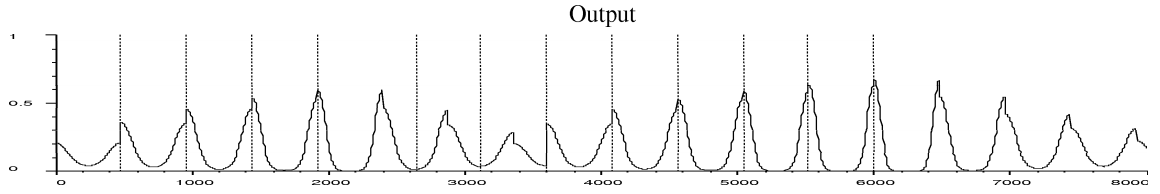
\includegraphics[scale=.3]{graph/BPM_large_oscillator}
            \end{figure}
            
            \begin{enumerate}
                \item	initialize pulse generator (tempo estimate, beat position estimate)
                \item<2->	predict next beat location with pulse
                \item<3->	adapt acc.\ to distance (predicted vs.\ real onset position)
                    \begin{itemize}
                        \item	beat period
                        \item	beat phase
                    \end{itemize}
                \item<4->	predict with adapted settings
                \item<4->   adapt \ldots
            \end{enumerate}
        \end{frame}
        \begin{frame}{tempo detection \& beat tracking}{oscillator approach: initialization}
            \question{How to estimate the initial tempo}

            \begin{itemize}
                \item	location of maximum of \textbf{ACF of novelty function}
                \item<2->	maximum of \textbf{IOI histogram}
                    \figwithmatlab{BeatHistogram}
                \item<2->	maximum of \textbf{beat spectrum/histogram}
                \item<2->	\ldots
            \end{itemize}
        \end{frame}
        \begin{frame}{tempo detection \& beat tracking}{multi-agent approach}
            \begin{enumerate}
                \item	run \textbf{multiple beat trackers} with different parameters
                    \begin{itemize}
                        \item	initial tempo
                        \item	initial beat phase
                        \item	adaptation speed
                    \end{itemize}
                \smallskip
                \item<2->	compute reliability/\textbf{confidence} criteria:
                
                    \begin{itemize}
                        \item	match beat and onset times
                        \item<3->	tempo stability
                        \item<4->	majority of different agents
                        \item   \ldots
                    \end{itemize}
                \smallskip
                \item<5->	choose\textbf{ most reliable agent} (or path between agents)
            \end{enumerate}
        \end{frame}
        
    \section{filterbank approach}
        \begin{frame}{tempo detection \& beat tracking}{filterbank approach}
            \begin{columns}[T]
            \column{.5\linewidth}
                \begin{enumerate}
                    \item	design \textbf{filterbank} (e.g. comb resonators spaced 1 beat)
                    \smallskip
                    \item<2->	compute filter output energy	
                    \smallskip
                    \item<3->	pick maximum
                \end{enumerate}
            \column{.5\linewidth}
                \only<1>{
                \begin{figure}
                    \centering
                        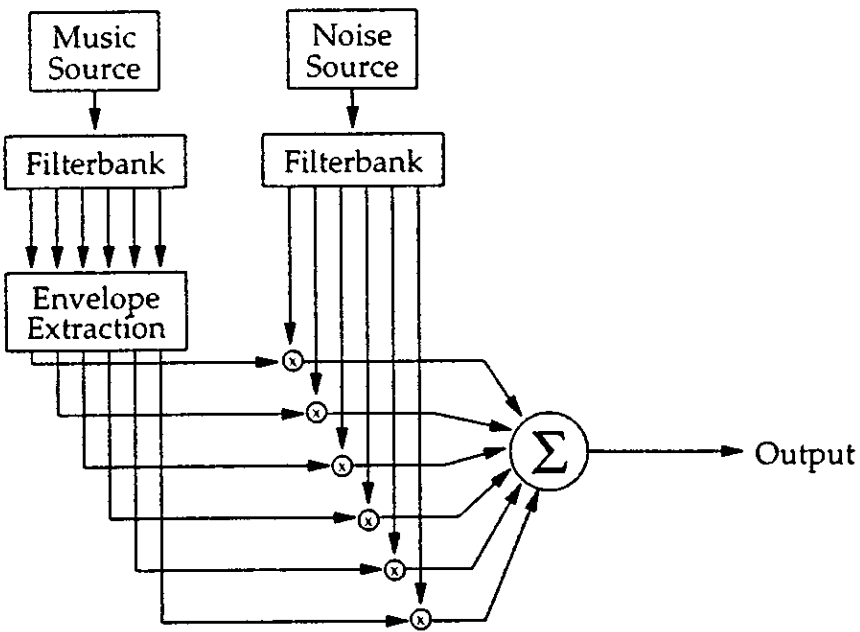
\includegraphics[scale=.25]{graph/BPM_Scheirer_filterbank}
                \end{figure}
                }
                \only<2->{
                \begin{figure}
                    \centering
                        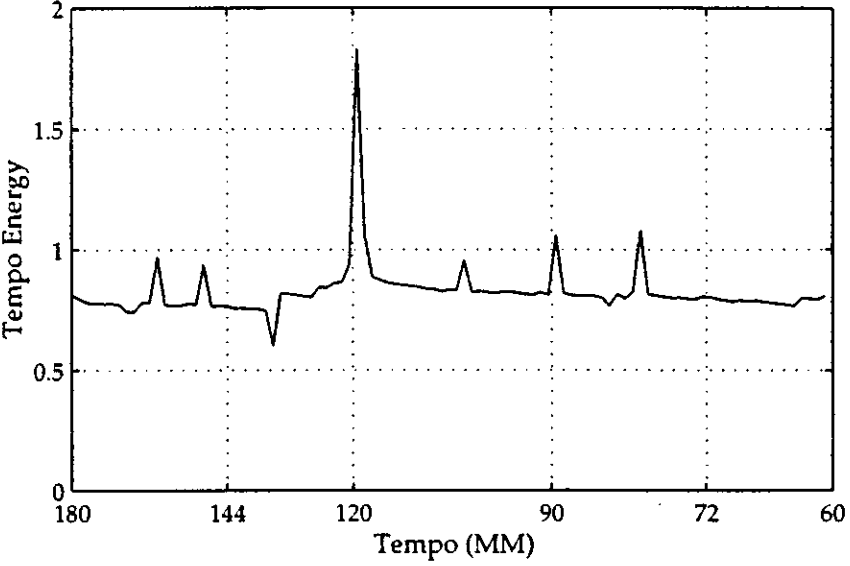
\includegraphics[scale=.25]{graph/BPM_Scheirer_beatspectrum}
                \end{figure}
                }
            \end{columns}
            plots by Scheirer\footfullcite{scheirer_tempo_1998}
        \end{frame}

    \section{template approach}
        \begin{frame}{tempo detection \& beat tracking}{template-based approach}
            \begin{enumerate}
                \item	define set of \textbf{template pulses} in all tempi
                \smallskip
                \item<1->	compute CCF between novelty function (or its ACF) and all templates
                \smallskip
                \item<1->	choose template with highest correlation as tempo
                \smallskip
                \item<1->	choose lag with highest correlation as beat phase
            \end{enumerate}
        \end{frame}

    \section{challenges}
        \begin{frame}{tempo detection \& beat tracking}{typical problems}
            \begin{enumerate}
                \item	tempo: detection of \textbf{double/half tempo} (triple, \ldots)
                \smallskip
                \item<1->	phase: detection of \textbf{off-beats}
                \smallskip
                \item<1->	tempo \& phase: strongly depends on \textbf{initialization values}
                \smallskip
                \item<1->	tempo \& phase: only \textbf{slow adaptation} --- no sudden tempo changes
            \end{enumerate}
            
            \bigskip
            example: challenges with adaptation speed\\                      \includeaudio{sonata-ck330_auftakt}
        \end{frame}
   
    \section[eval]{evaluation}
        \begin{frame}{tempo detection \& beat tracking}{evaluation}
            
            \begin{itemize}
                \item   evaluation of \textbf{constant tempo }
                    \begin{itemize}
                        \item   match within tempo range $\Rightarrow$ classification metrics
                    \end{itemize}
                \smallskip
                \item<2->   evaluation of \textbf{beat tracking }
                    \begin{itemize}
                        \item   ground truth can be subjective (double/half tempo, deviations)
                        \item   each beat matched against ground truth 
                            \begin{itemize}
                                \item   challenge 1: tolerance window definition (tempo dependent or not?)
                                \item   challenge 2: slightly different tempo might lead to gap between metrics and perceptual severity
                            \end{itemize}
                    \end{itemize}
                \smallskip
                \item<3->   \textbf{typical errors}
                    \begin{itemize}
                        \item   double/half tempo (sometimes also 3/2 relationships)
                        \item   off-beat
                        \item   problems with abrupt tempo changes
                    \end{itemize}
            \end{itemize}
        \end{frame}
    
    \section{summary}
        \begin{frame}{summary}{lecture content}
            \begin{itemize}
                \item   \textbf{tempo analysis}
                    \begin{itemize}
                        \item   similar to pitch detection on a different scale
                            \begin{itemize}
                                \item   periodicity analysis of novelty function
                                \item   time or spectral domain
                            \end{itemize}
                    \end{itemize}
                \bigskip
                \item   \textbf{typical approaches}
                    \begin{itemize}
                        \item   oscillator
                        \item   histogram/beat spectrum
                        \item   template correlation
                    \end{itemize}
                \bigskip
                \item   \textbf{main challenges}
                    \begin{itemize}
                        \item   double/half tempo
                        \item   adaptation to sudden tempo changes
                    \end{itemize}
            \end{itemize}
            \inserticon{summary}
        \end{frame}
\end{document}
